\section{Analyse de l'existant}

\subsection {Présentation générale}
Actuellement le savoir-faire est très limité, en effet il y a peu de processus de gestion déclenchés pour surveiller les sites. Le schéma ci-dessous résume la surveillance actuelle.\\

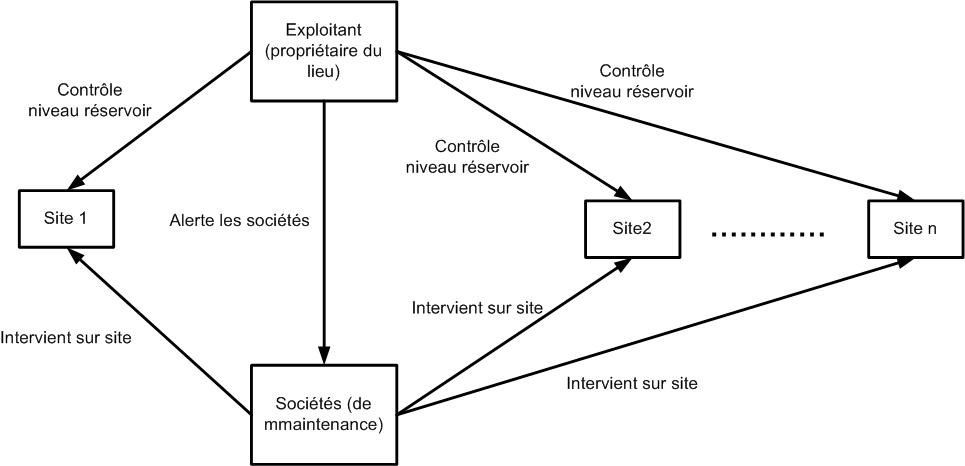
\includegraphics[width=0.9\textwidth]{img/schemaAnalyseExistant.png}

~\\
Le matériel est celui utilisé par les sociétés de maintenance intervenant sur les sites (camions, systèmes de vidage/remplissage..)
Deux métiers ont été identifiés, les propriétaires des sites s’occupent de leur exploitation tandis que les sociétés spécialisés sont chargées du métier de la maintenance.

\subsection {Contexte géographique}

COPEVUE gère actuellement de nombreux sites isolés concernés par le système à mettre en place. Ils peuvent être situés aussi bien dans les pays Nordiques de l'UE que dans certaines régions méditerrannéennes. La principale caractéristique de ces sites est leur isolement : ils sont généralement dans des régions peu peuplées et sont difficiles à atteindre. \\
Le premier déploiement de la solution proposée à cette appel d'offre s'effectuera dans la partie Nord de la Norvège.


\subsection {Fonctionnement actuel}

Le contrôle des sites isolés est actuellement effectué directement leur propriétaire. Ils doivent se rendre sur chacun de leurs sites afin d'effectuer les vérifications appropriées et appeler la société spécialisée chargée de la maintenance du site si nécessaire.\\
Nous pouvons aisément constater en observant le mode de fonctionnement actuel son manque d'efficacité, de fiabilité et d'économie de ressources. En effet, faire se déplacer les propriétaires à intervalles réguliers sur leurs sites est très coûteux en temps de trajets (certains propriétaires possèdent de nombreux sites éloignés les uns des autres). Ces déplacement engendrent un coût non négligeable en raison des distances à parcourir. \\
La fiabilité des tests est également relativement faible en raison de l'intervalle de temps entre deux mesures sur une même cuve, celle-ci pouvant nécessiter une maintenance urgente si le niveau d'une cuve atteint un seuil critique. Un contrôle, même régulier des propriétaires ne permet pas de détecter le dépassement du seuil critique dans un délai suffisamment court.\\
Enfin, lorsque les propriétaires signalement un besoin de maintenance à une entreprise spécialisée, il est impossible à l'heure actuelle, de savoir si un autre site à proximité aurait un besoin similaire. Les camions chargés de la maintenance des différents sites sont donc sous-exploités et sont contraints d'effectuer de nombreux allers-retours entre les différents sites et leur base.

\subsection {Existant informatique}

COPEVUE n'a actuellement aucune gestion informatique centrale des différents sites isolés.
